% !TeX spellcheck = en_GB
\section{Optimal Estimation Retrieval Algorithm} %Section - 1.2
\label{sec:retrieval}
The purpose of this study is to apply an optimal-estimation snowfall retrieval on ground based measurements to estimate the surface accumulation and vertical snow water content for an extreme event during Christmas 2016. These will later be used to compare to \SI{48}{\hour} MEPS model forecasts to see if the model was able to predict synoptical features and precipitation related to the extreme event 'Urd' in 2016. 
% maybe start out by saying that you are trying to estimate atmospheric parameters  (SWC in our case) from a set of measurements.   The optimal-estimation approach provides a flexible retrieval framework that can incorporate multiple measurements/ pieces of information into a common retrieval framework.  In this way, we can use measurements from MRR, PIP, and MASC to estimate vertical profiles of snowfall.  You could then discuss the reindeer -> tracks thing to illustrate the general principle.  
% literally taken from paper until Skofronick, Noh
The quantitative estimation of snowfall at the global scale from spaceborne measurements has been available only recently. Initial retrieval approaches were based on passive microwave measurements \citep{skofronick-jackson_physical_2004,noh_development_2006}. But since these passive measurements can only assess total integrated snow water path for a given column, such efforts were unable to provide much information on the profiles of snow water content. 
The launch of the CloudSat \SI{94}{\giga\hertz} Cloud Profiling Radar (CPR) in 2006, however, provided the first opportunity to examine such vertical structure at a global scale. 
%Several studies, such as \citet{matrosov_modeling_2007} and \citet{kulie_utilizing_2009}, have shown that the CPR can be used to estimate snofall rate but that estimated snowfall values depend heavily upon assumed snowflake microphysical properties. 
Several studies have shown, that estimated snow rate depends upon retrieval assumptions such as snowflake habit and particle size distribution (PSD) and can give large differences for a given radar reflectivity.
\\
For the operational CloudSat snowfall retrieval scheme (2C-SNOW-PROFILE), \citet{wood_microphysical_2015} developed snowflake particle models based upon video snow disdrometer observations from the Canadian CloudSat-CALIPSO Validation Project \citep[C3VP,][]{hudak_canadian_2006}. Scattering properties for these snow particle models were based upon the Discrete Dipole Approximation (DDA) method. 
%It was hoped that the use of realistic snow properties in the retrievals would lead to reasonable estimates of snowfall in the retrieval. 
In addition, they derived an a priori relationship between particle size distribution and temperature that they could use as an additional constraint for the snowfall scheme. Use of the flexible optimal-estimation retrieval framework allowed to develop a best estimate of snow properties that are consistent with both the CPR reflectivities and the a priori constraint. 
\\
They have also been used to estimate snowfall in remote locations such as the Antarctic and Arctic \citep{palerme_how_2014,kulie_shallow_2016} that in turn have been used to evaluate the representation of snowfall in climate models \citep{palerme_evaluation_2017,christensen_arctic_2016}. 
These estimates have been used to assess the performance of ground-based radar schemes such as those based upon the operational weather radar system in Sweden \citep{norin_intercomparison_2015}. Despite such progress, however, the CloudSat scheme can still lead to uncertainties in the retrievals of up to \SIrange{140}{200}{\percent} \citep{wood_estimation_2011} for individual storms.
\\
Again, these uncertainties arise from the large variance in snowflake microphysical  properties as observed in nature. In response, \citet{cooper_variational_2017} explored the use of in-situ, event specific  observations of snowflake microphysical properties to improve radar-based retrievals of snowfall. This work was based upon observations from the Ka-band ARM (The Atmospheric Radiation Measurement) Zenith Radar (KAZR) and Multi-Angle Snow Camera (MASC) deployed at the ARM Climate Facility Site at Barrow, Alaska in Spring 2014. This ground-based \SI{35}{\giga\hertz} retrieval scheme was modified from the space-borne \SI{94}{\giga\hertz} CloudSat retrieval scheme developed by \citet{wood_estimation_2011}. But instead of using a temperature dependent a priori characterisation of PSD, \citeauthor{cooper_variational_2017} introduced the in-situ observations of particle size distribution through the a priori terms of the optimal-estimation framework. 
\\
%
Preliminary analyses suggested good performance for this retrieval scheme at Barrow, Alaska. Estimates of snowfall from the \citet{cooper_variational_2017} approach differed by \SI{18}{\percent} relative to nearby National Weather Service snow gauge measurements for total accumulation over multiple snow events. However, given limited snowfall observed at Barrow during the deployment of the MASC, it was difficult to come to any definitive conclusions about retrieval performance. The NSF (National Science Foundation) funded field campaign with MRR, MASC, and PIP (Precipitation Imaging Package) deployment at Haukeliseter provides an ideal opportunity to further explore the \citet{cooper_variational_2017} retrieval approach. This thesis will continue to examine the sensitivity of retrieval surface snowfall rate to assumptions of habit, fall speed, and particle size distribution as in \citet{cooper_variational_2017}. In addition, this study here will will examine the vertical profiles of snowfall profiles in the atmospheric column.
%%%%%%%%%%%%%%%%%%%%%%%%%%%%%%%%%%%%%%%%%%%%%%%%%%%%%%%%%%%%%%%%%%%%%%%%%%%%%%%%%%%%%%%%%%%%

%%%% OE scheme %%%%%%%
\subsection{Snowfall Retrieval Scheme}\label{sec:ret_scheme}
%%% image forward problem %%%%%%%%%%%%%%%%%%%%%%%%%%%%%%%%%%%%%
% !TeX spellcheck = en_GB
\begin{wrapfigure}[17]{r}{0.44\textwidth}
	\vspace{-\normalbaselineskip}
	\centering
	\begin{subfigure}[b]{0.4\textwidth}
		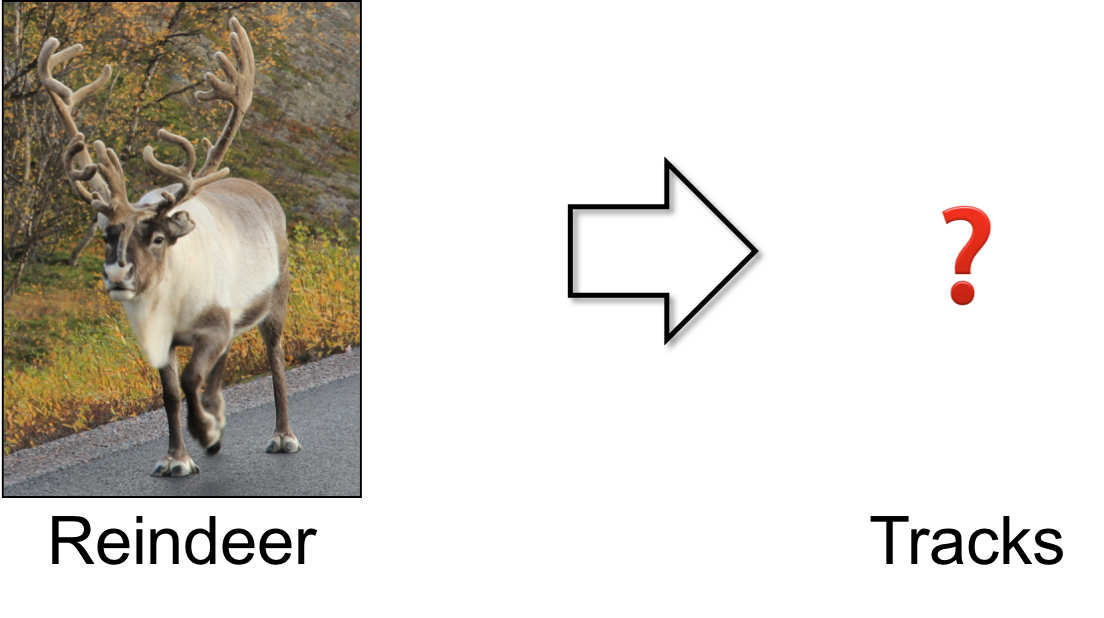
\includegraphics[trim={0cm, 0cm, 0cm, 0cm},clip,width=\textwidth]{./fig_instruments/Forward_problem.png}
		\caption{Forward problem.}\label{fig:dragon:forward}
	\end{subfigure}
	
	\begin{subfigure}[b]{0.4\textwidth}
		
\includegraphics[trim={0cm, 0cm, 0cm, 0cm},clip,width=\textwidth]{./fig_instruments/Inverse_problem.png}
		\caption{Inverse problem.}\label{fig:dragon:inverse}
	\end{subfigure}
	\caption{\protect\subref{fig:dragon:forward}: Forward problem, relationship between parameter of interest (reindeer) and the unknown parameter of measurements (tracks). \protect\subref{fig:dragon:inverse}: An inverse problem when the parameter of measurements is known, but the parameter of interest is not \citep{stephens_remote_1994}.}\label{fig:dragon}
	\vspace{-\normalbaselineskip} 
\end{wrapfigure}


%%%%%%%%%%%%%%%%%%%%%%%%%%%%%%%%%%%%%%%%%%%%%%%%%%%%%%%%%%%%%%%%%%%%%%%%%%
The optimal-estimation snowfall retrieval scheme was modified for the Barrow instrumentation described in \citet{cooper_variational_2017} to the \SI{24}{\giga\hertz} MRR, MASC, and PIP located at Haukeliseter. This scheme was then used to derive surface snowfall rates and vertical profiles of snow water content using different combinations of retrieval assumptions based upon in-situ observations.
Here a discussion of the optimal-estimation framework is presented so that the reader can understand exactly how the different measurements in the retrieval scheme were incorporated. The differences in the forward and inverse problem are reviewed in the beginning. Both, forward and inverse problem underlie the basic methodologies of remote sensing.
\\
\\
The general concepts of forward and inverse problems are illustrated in \Cref{fig:dragon}.  The forward problem describes the relationship between the physical parameters of interest and the measurements (\Cref{fig:dragon:forward}). In \Cref{fig:dragon:inverse}, the physical parameter is the reindeer and the measurements are its tracks. In the here presented thesis snowfall scheme, the physical parameters are the vertical profiles of snow water content (SWC) and the measurements are the MRR reflectivities.  The inverse problem represents the opposite goal.  The physical entity (reindeer and SWC) must be inferred from the measurements (reindeer tracks or MRR reflectivities).
\\
\\
The optimal-estimation framework is used to solve the inverse problem for the thesis work. But it is more complex than the direct inversion as represented in \Cref{fig:dragon:inverse}. Instead of inverting directly for the parameter of interest (SWC) from the measurements [\SI{}{\decibel ze}], the scheme includes additional information based upon an 'a priori' understanding of the physics of the retrieval problem. Thus, it represents a weighted balance between what the data can tell about the state and what is already known about it. For the CloudSat retrieval scheme, this a priori information came from a parametrisation relating particle size distribution (PSD) to temperature. For the Barrow and Haukeliseter schemes, the a priori information could also come from the in-situ observations of snowflake microphysics. These constraints also add numerical stability to the inversion process when there are either calibration errors in the measurements or uncertainties in the forward model that relates the physical parameter to measurement space. Details of the radar forward model are discussed at the end of this section.
\\
\\
The optimal estimation method is based on Gaussian statistics.  It solves for snowfall properties of interest or retrieval vector, $\mathbf{x}$, by minimizing the scalar cost function, $\Phi$ , as in \Cref{eq:scalar_cost_fct}.
\begin{equation}
\begin{split}
\Phi(\mathbf{x},y,a) = & (y- F(\mathbf{x}))^T \mathbf{S}_y^{-1} 			(y-F(\mathbf{x})) \\
&+(\mathbf{x}-a)^T \mathbf{S}_{a}^{-1} (\mathbf{x}-a)
\end{split} \label{eq:scalar_cost_fct}
\end{equation}
Specifically, or this thesis retrieval scheme, $\mathbf{x}$ represents the PSD parameters of slope and number intercept of an assumed exponential size distribution for each radar range bin as in \Cref{eq:num_dens}. $y$ is the vector of MRR reflectivites. The vector $a$ is the a priori guess for slope parameter and number in each range bin. $F(\mathbf{x})$ represents the forward model that translates snow properties into reflectivity space.  Minimizing the cost function therefore seeks to reduce the difference between the observations, $y$, and simulated observations, $F(x)$ and between the a priori guess ($a$) and the retrieval vector ($x$).
\begin{align}
	n(r) & = N_{0} \exp\left(-\lambda r\right) \qquad [ \SI{}{\per\cubic\metre\per\mm} ] \label{eq:num_dens}
\end{align}
The $\mathbf{S}_y$ and $\mathbf{S}_{a}$ terms, in \Cref{eq:scalar_cost_fct}, represent the forward model and measurement error covariance matrix and the a priori error covariance matrix, respectively. The relative differences between $\mathbf{S}_{a}$ and $\mathbf{S}_y$ weight the importance of the observations and the a priori considerations in determining our best estimate of PSD properties. 
\\
\\
Newtonian iteration is used until the value of the cost function converges and our best estimate of snowfall properties are found.  The optimal-estimation scheme also provides error diagnostics through the retrieval error covariance matrix, $\mathbf{S}_x$, as in \Cref{eq:Sx}.
\begin{align}
	\mathbf{S}_x & = \left( \mathbf{S}_a^{-1} + \mathbf{K}^T \mathbf{S}_y^{-1} \mathbf{K} \right)^{-1}\label{eq:Sx}
\end{align}
The Jacobian matrix, $\mathbf{K}$, represents the sensitivity matrix of the perturbed result of the forward model. The true state $\mathbf{x}$ is perturbed by \SI{0.2}{\percent} and thus $\mathbf{K}$ represents the relation between simulated values to the true state and how sensitive the simulated values are to small changes when starting a new retrieval cycle. The closer $\mathbf{K}$ is diagonal, the more is $\mathbf{x}$ determined by the real observed and a priori values. If the limit of the partial derivative is close to unity, the retrieved value $\mathbf{x}$ is its true state \citep{wood_estimation_2011}.
\\
\\
In practical application for this multiple layer retrieval scheme, log-transformed particle size distribution parameters of slope and number intercept were used due to the large expected range of these variables. The state vector, $\mathbf{x}$, is defined in \Cref{eq:snow_prop}.
\begin{align}
	\mathbf{x} & = \begin{bmatrix}
		log(\lambda)_0 	\\
		\vdots 			\\
		log(\lambda)_{\text{nlayer}} 	\\
		log(N_0)_0		\\
		\vdots			\\
		log(N_0)_{\text{nlayer}}		
	\end{bmatrix} \qquad \text{nlayer} = 14
	\label{eq:snow_prop}
\end{align}
The usage of a priori terms were explored both from in-situ microphysical observations and from the PSD-temperature relationship developed for the CloudSat scheme as in \Cref{eq:lambda,eq:N0}. Temperatures in \SI{}{\celsius} at Haukeliseter were taken from site measurements with an assumption of a moist adiabatic lapse rate for the observed snow events. The log transformed slope and number intercept values were taken from \citet{wood_estimation_2011}. 
\begin{align}
	\log(\lambda) & = -0.03053 \cdot T_{ap} - 0.08258  \label{eq:lambda} \qquad [ \log(\SI{}{\per\mm}) ] \\
	\log(N_0) & = -0.07193 \cdot T_{ap} +2.665  \qquad [ \log(\SI{}{\per\cubic\metre\per\mm})]
	\label{eq:N0}
\end{align}
The log-transformed equations are useful, since the results from C3VP were similar to other observations. The study showed, that $N_0$ ranges over several order of magnitude as well as $\lambda$ was non-Gaussian for the snow events \citet{wood_estimation_2011}. The diagonal matrix elements in $\mathbf{S}_a$ (\Cref{eq:scalar_cost_fct,eq:Sx}) are equal to \numlist{0.133;0.95} for the particle slope parameter and the number intercept, respectively, as from Eq. 7.35 and 7.36 in \citet{wood_estimation_2011}. The diagonal matrix elements for $\mathbf{S}_y$ are $2.5^2$ in \Cref{eq:scalar_cost_fct,eq:Sx}.
\\
\\
After the best estimate of PSD parameters are found, the snow water content in each layer is calculated using the snow particle mass-dimension relationships as in \Cref{app:scat_scheme}. 
%
\begin{align}
	\text{SWC} & = \int_{r_{min}}^{r_{max}} m(r) n(r) dr \qquad [\SI{}{\gram\per\cubic\metre}] \label{eq:SWC}
\end{align}
$r$ is the particle maximum dimension and $m(r)$ the related mass. 
\\
This thesis work considered the database of particle models developed for the CloudSat mission, e.g. different types of aggregates, sector plates, and columns. Scattering properties for these snowflakes were calculated for the \SI{24}{\giga\hertz} frequency using discrete dipole approximation (DDA). Observations from the MASC of snowflake habit were used to guide particle selection. Snow water content, in turn, was translated into a snowfall rate using fall speed observations (MASC, PIP, or MRR Doppler velocity) or climatological analyses ($V = \SI{0.85}{\mPs}$). Surface snowfall rate is estimated using the SWC from the lowest non-noise reflectivity and radar bin. 
\\
\\
The forward model that calculates simulated \SI{24}{\giga\hertz} MRR reflectivities from PSD parameters was modified from that used in the CloudSat \SI{94}{\giga\hertz} operational snowfall product (2C-SNOW-PROFILE). Backscatter from frozen hydrometeors in each radar bin is summed up as in \Cref{eq:backscatter} form which reflectivity factor, Z, can be found (\Cref{eq:singleZ}). 
% singly-scattered non-attenuated reflectivity
\begin{align}
	\eta_{bk} & = \int_{r_{min}}^{r_{max}} n(r) \sigma_{bk} dr \qquad [\SI{}{\per\metre}] \label{eq:backscatter} \\
	Ze^{ss,na} & = \frac{\Lambda^4}{\left\| K_w \right\|^2 \pi^5} \eta_{bk} \qquad [\SI{}{\mm^6\metre^{-3}}] \label{eq:singleZ}
\end{align}
where, $\Lambda$ is the wavelength of the radar; $\left\| K_w \right\|^2$ is the complex refractive index of water. Radar backscatter values were estimated using discrete dipole approximation for the CloudSat particle models at \SI{24}{\giga\hertz}. Unlike the \SI{94}{\giga\hertz} spaceborne CloudSat mission, multiple scattering and attenuation can be neglected for \SI{24}{\giga\hertz} MRR and the short path length retrievals as viewed from the ground perspective.  

%\newpage
\subsection{Environmental Masks for the Optimal Estimation Retrieval}\label{sec:pre_snow}
%%% image surface temperature and MRR %%%%%%%%%%%%%%%%%%%%%%%%%%%%%%%%%%%%%
% !TeX spellcheck = en_GB
\begin{figure}[t!]
	\centering
	%    \begin{subfigure}[b]{\textwidth}
	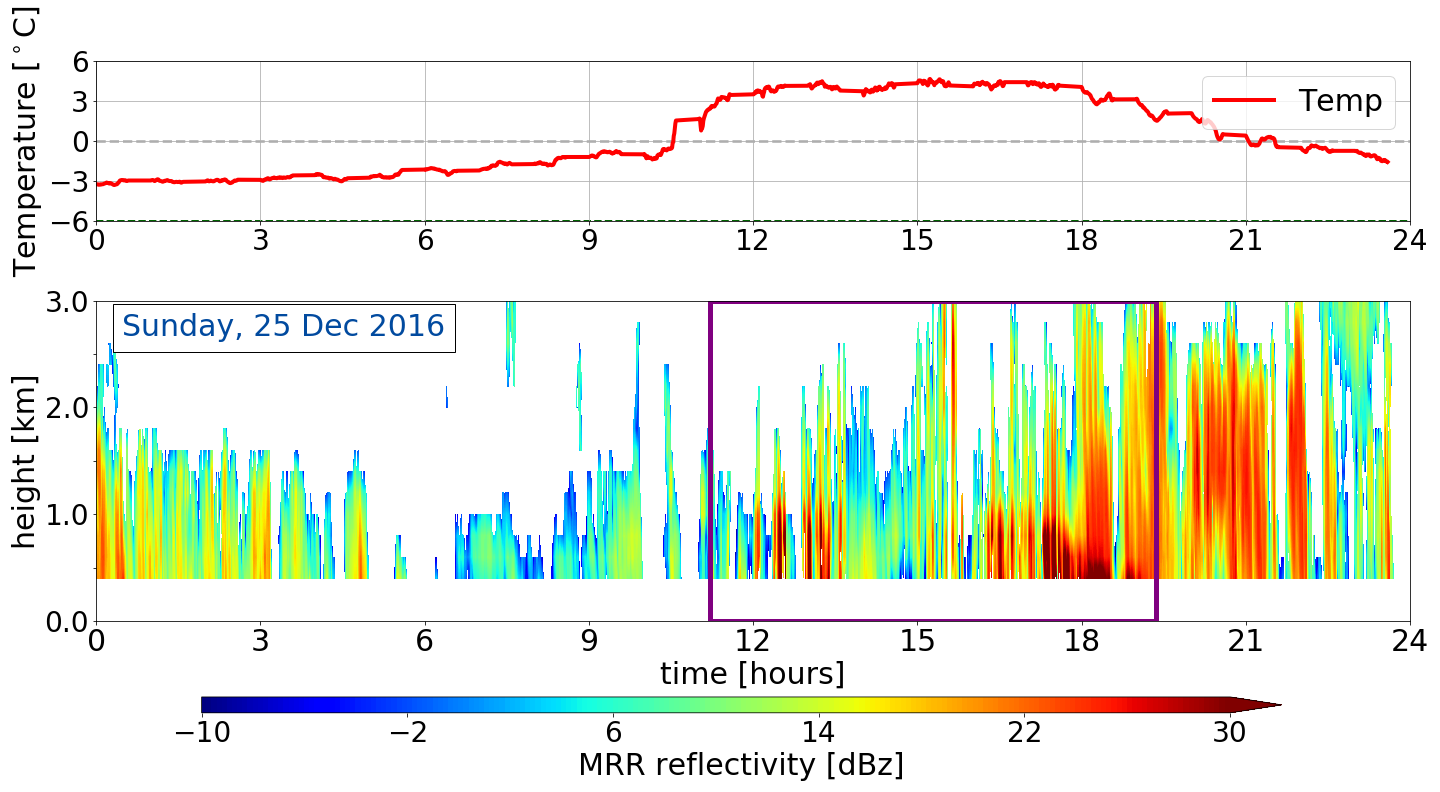
\includegraphics[width=\textwidth]{./fig_MRR/MRR_sfcT_20161225}
	%	\end{subfigure}
	\caption{A priori temperature dependence within the optimal estimation retrieval for an all day precipitation event on \SI{25}{\dec}. The upper panel shows the surface a priori guess, $T_{ap}$, measured at the Haukeliseter site. The lower panel presents the reflectivity measure by the MRR. Additionally, indicates the purple frame the time, where the MRR reflectivity was larger than \SI{-10}{\dB Z} and surface temperatures less than \SI{2}{\celsius} }\label{fig:MRR_sfcT}
\end{figure}
%%%%%%%%%%%%%%%%%%%%%%%%%%%%%%%%%%%%%%%%%%%%%%%%%%%%%%%%%%%%%%%%%%%%%%%%%%
\noindent
Different steps and assumptions are done in the here presented snowfall retrieval, to achieve vertical profiles of snowfall from MRR. The snowfall rate at the surface can be estimated from one of the lower levels. The optimal estimation retrieval is only performed for profiles, which are likely to have observed snow. 
%Relationships between reflectivity and snowfall have been developed in previous studies. Different crystal shapes led to different results, even if the PSD of ice particles is known. Snow densities vary significantly from storm to storm, where small particles are still Rayleigh scattered, and larger particles non-Rayleigh scattered \citep{gunn_microwave_1954}. 
\\
This value was  chosen as sensitivity studies \citep[e.g.][]{wood_level_2013} that a days worth of such reflectivities would produce only a trace of snow.  Such a value therefore guarantees that a significant snow event is not missed and that any storms with lower \SI{}{\decibel Z} values would not produce meaningful precipitation.
%A reflectivity threshold of \SI{- 15}{\decibel Z} was selected for the scheme. The threshold is similar to the one used in \citet{wood_level_2013}. Light liquid precipitation is related to \SI{- 10}{\decibel Z} \citep{stephens_properties_2007}. \citet{wood_estimation_2011} found, that the reflectivity above \SI{-15}{\dB Z} are not influenced by ground clutter, when the reflectivity in the lowest bin and adjacent bin is compared.
\\
The Haukeliseter measurement site is equipped with a weather mast, measuring the air temperature every minute at two-meter height (compare \Cref{fig:MRR_sfcT}, upper panel). 
%
Since the MRR measures above \SI{300}{\metre} and temperature measurements exists only at the surface, a priori temperature ($T_{ap}$) at the surface is assumed to be similar to the observed near-surface air temperature. The use of a moist adiabatic lapse rate of $dT/dz = \SI{5}{\kelvin\per\km}$ gives $T_{ap}$ in each layer. 
Snow existence at temperature measurements up to a threshold of +\SI{2}{\celsius} are assumed. \citet{liu_g._deriving_2008} validated this threshold, by analysing present weather reports to find the distinction between liquid and solid precipitation.\\
The purple line in the lower panel of \Cref{fig:MRR_sfcT} represents the time frame during \SI{25}{\dec}, where the MRR reflectivity is less than \SI{- 15}{\decibel Z}, and a priori temperature passes the \SI{2}{\celsius} limit at the surface.  
